\chapter{Background}
This chapter offers the technical background related to the research question of this work. We start by providing a comprehensive overview of \gls{nas} and introduce the three dimensions that characterize a \gls{nas} algorithm, followed by an anatomy of the high-performing search algorithm \gls{bananas}. Then, we review the existing uncertainty quantification techniques, with a focus on \gls{cp} algorithms, particularly those related to the novel framework we propose in Chapter~\ref{ch3}.

\section{Neural Architecture Search}
\subsection{Overview}
\label{sec: nas}
In the recent decades, deep learning has achieved remarkable success in a variety of areas, including computer vision, natural language understanding, and machine translation. This success is partly attributed to the carefully designed neural network architectures. With the rising demand for efficient architecture engineering in complex domains, \gls{nas} has emerged as a technique for automating the design of neural architectures for specific tasks.
 
\gls{nas} has been a rapidly progressing research domain in the past years. Since the seminal work that achieves competitive performance on CIFAR-10 \cite{zoph2017neural}, numerous \gls{nas} algorithms built on different techniques have been proposed. In general, \gls{nas} algorithms can be characterized by three key dimensions: search space, search strategy, and performance evaluation strategy \cite{elsken2019neural, white2023survey, wistuba2019survey}. Figure \ref{fig: nas_overview} illustrates a typical architetcture search process.


\begin{figure}[htbp]
	\centering
	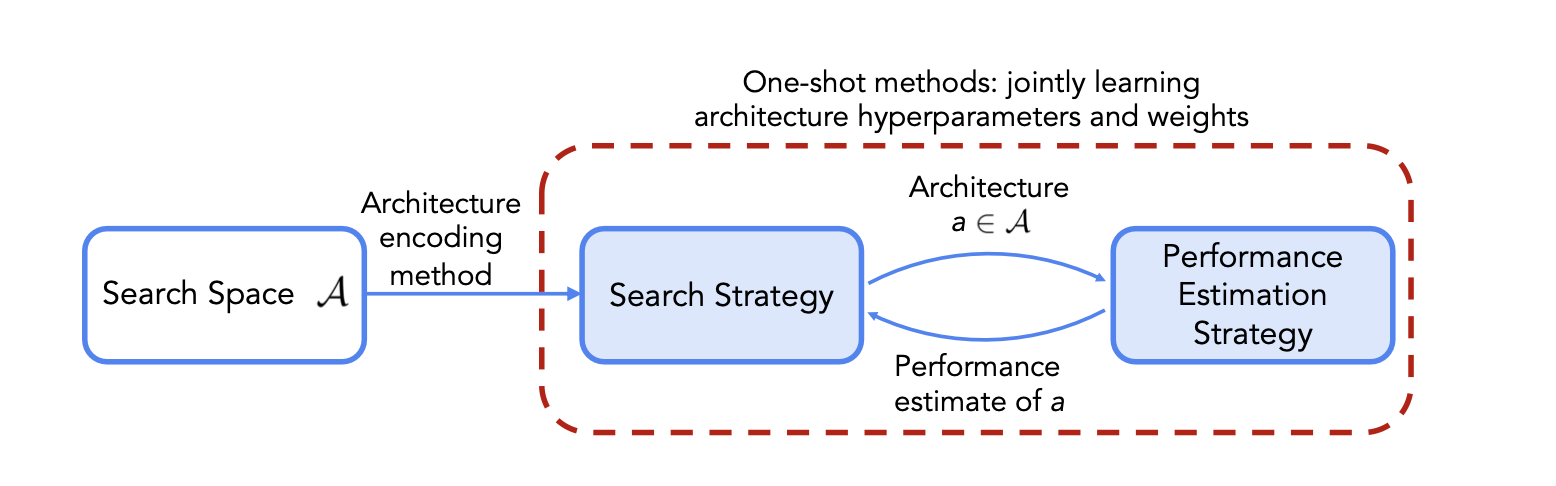
\includegraphics[scale=0.5]{figs/overview_nas.png}
	\refstepcounter{figure}
   	\addcontentsline{lof}{figure}{Figure~\thefigure: Overview of Neural Architecture Search}
	\label{fig: nas_overview}
	\parbox{\linewidth}{
	 \vspace{0.5em}
 	 {\small \textit{Figure \ref{fig: nas_overview}:} Overview of an architecture search process. The search strategy iteratively selects architectures from a predefined search space $\mathcal{A}$. The performance estimation strategy evaluates the model performance on the target dataset and then communicates back the performance to the search strategy.  \cite{white2023survey}.
	}
 	}
\end{figure}

\noindent Next, we provide definitions of the terms and review the research progress of each domain.
\begin{description}[leftmargin=0cm, listparindent=\parindent]
	\item [Search Space] A search space defines a set of architectures that the search algorithm is allowed to select. The search space is often the first step when setting up \gls{nas} and perhaps is also the most essential step, because
		the design of the search space represents an important trade-off between human bias and efficiency of search: a
		smaller search space incorporating more prior human knowledge and involving more manual decisions will enable
		\gls{nas} algorithms to find high-performing architectures more easily, in contrast a larger space with more primitive
		building blocks provides higher odds of discovering truly novel architectures \cite{white2023survey}. Common  search
		spaces range in size from a few thousand to over $10^{20}$.	
	
		There are four major categories of search spaces in the \gls{nas} literature \cite{white2023survey}. We start with two types of search spaces that have relatively simple architecture topologies. The macro search spaces \cite{baker2017designing, kandasamy2018neural, zoph2017neural} encode the entire neural architecture at a high level. Typically, an entire architecture is often represented by a \gls{dag}, with nodes defining the operation types and edges representing data flows. Each node is allowed to have distinct structures, such as convolution, pooling. As a result, macro search  spaces are highly flexible and possess high representation power. Another type is the chain-structured search spaces. As suggested by the name, chain-structured search spaces consist of neural networks that can be written as a sequence of operation layers. These search spaces often take state-of-the-art manual designs as the backbone. For example, there are several chain-structured search spaces based on the convolutional networks \cite{cai2018proxylessnas} or the transformer architectures \cite{xu2021nasbert}. 
		
		The third group is the cell-based search spaces, which perhaps are the most popular type of search spaces in \gls{nas} research. The cell-based search spaces are inspired by the fact that state-of-the-art human-designed architectures often consist of repeated blocks. For instance, the high-performing Transformer \cite{vaswani2017attention} contains 6 identical stacked encoder and decoder layers. Thus, instead of searching for the entire network architecture from scratch, \cite{zoph2018learning} propose to only search over relatively small cells  that comprises a set of operations, such as convolution. Then, the overall architecture can be formed by stacking the cells following a predefined skeleton. Building on this idea, \cite{zoph2018learning} proposes the first modern cell-based search space, NASNet, which comprises of two types of cells: the normal cell that preserves the dimensionality and the reduction cell that reduces the spatial dimension, as illustrated in Figure \ref{fig: cellss}. Since its emergence, many other cell-based search spaces have been developed. In general, these cell search spaces share a high-level similarity, but differ in the design of the fixed macro structure, the layout and constraints in the cells, and the choices of operations within the cells \cite{dong2020nasbench201, liu2018darts,  pmlr-v97-ying19a}. The cell-based approach significantly reduces the size and the complexity of the search space. However, it has been criticized for limiting the expressiveness of \gls{nas}, potentially hindering the discovery of highly novel architectures \cite{white2023survey}.	
		
		\begin{figure}[htbp]
			\centering
			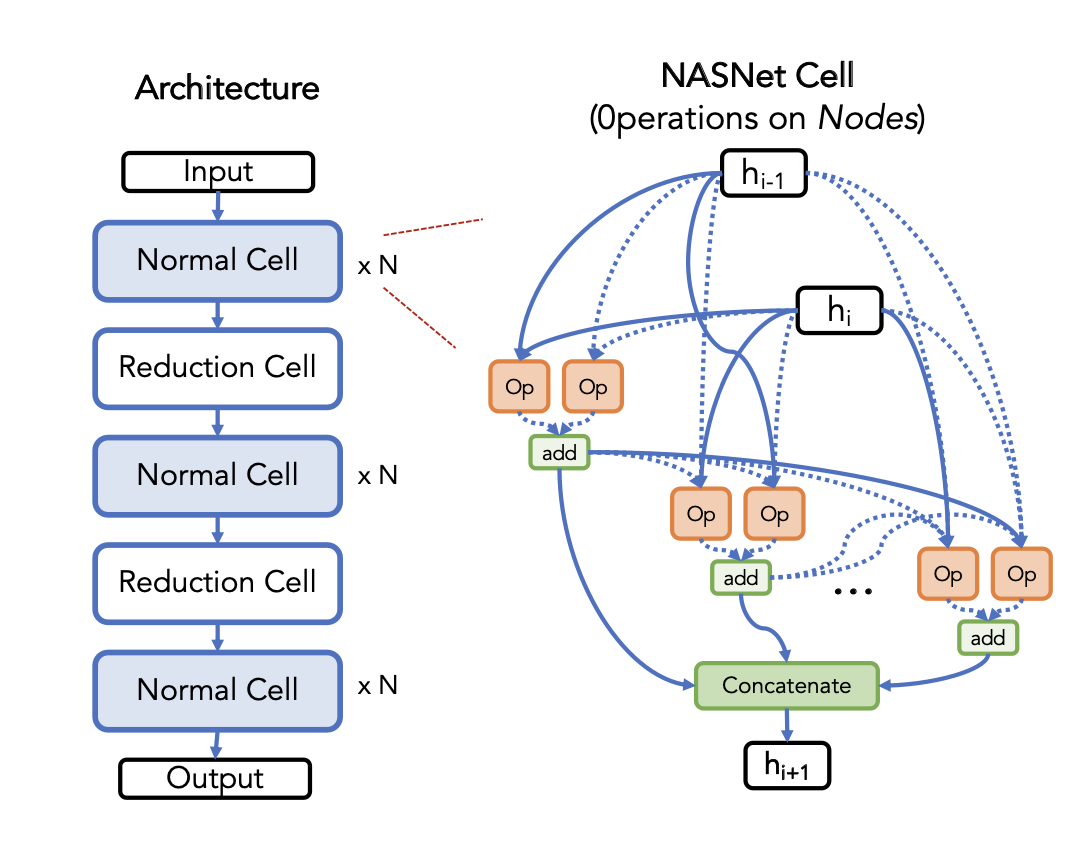
\includegraphics[scale=0.45]{figs/overview_cell_based_ss.png}
			\refstepcounter{figure}
   			\addcontentsline{lof}{figure}{Figure~\thefigure: Overview of Cell-based Search Space}
			\label{fig: cellss}
			\parbox{\linewidth}{
	 		\vspace{0.5em}
 	 		{\small \textit{Figure \ref{fig: cellss}:} Overview of a cell-based search space NasNet. The outer skeleton across cells (left) is fixed, and the operations, represented by nodes, within the cells are searchable (right) \cite{white2023survey}.
			}
 		}
		\end{figure}
		
		The last main category is the hierarchical search spaces. Different from the aforementioned types of search spaces that mostly have a flat representation, hierarchical search spaces involve designing patterns at different levels, where each higher-level pattern is often represented as a \gls{dag} of lower-level patterns \cite{christoforidis2021novel, liu2018hierarchical}.
		
	In addition to the architecture topology, another important design accompanying a search space is architecture encodings, because  many \gls{nas} algorithms require representations of the architectures to, for example, mutate an architecture or train a predictive model to extrapolate its performance. For search spaces that can be represented by a \gls{dag}, adjacency matrix is a commonly used encoding method. In addition, other encoding techniques, including graph-based encoding \cite{ning2020generic}, path-based encoding \cite{white2019bananas} and conditionally-structured encoding methods tailored for hierarchical search spaces have been proposed. \cite{white2020study} has shown that the effect of the encoding methods varies across different \gls{nas} subroutines.	
	  
	\item [Search Strategy] According to \cite{white2023survey}, there are generally two main categories of search strategies: black-box optimization based techniques and one-shot techniques. 
	 
		The black-box optimization based techniques largely overlap with another sub-area of AutoML: the hyperparameter tuning. Common techniques for hyperparameter tuning have been proven efficient for \gls{nas} as well, including reinforcement learning \cite{zoph2017neural, zoph2018learning}, evolutionary algorithms \cite{maziarz2018evo-nas,  real2019regularized}, gradient descent\cite{liu2018darts}, and etc. In particular, we take a close look at the search strategies based on Bayesian optimization, since they are closely related to the research question of this work. Initial Bayesian optimization based \gls{nas} approaches typically use the Gaussian Process (GP) as the surrogate model \cite{kandasamy2018neural}. However, these algorithms often demonstrate under-performance compared to their competitors due to several limitations: 1) search spaces are usually high-dimensional, non-continuous, and graph-like; 2) GPs requires custom distance metrics among architectures, which involves a time-consuming matrix inversion step. Besides, GPs are difficult to scale since the computation complexity grows cubically with the number of observations. To address these challenges, a new framework that using a neural predictor as the surrogate model for Bayesian optimization has been proposed and demonstrated strong performance \cite{ma2019deep, springenberg2016bayesian, white2019bananas}. We review this framework in details in Section \ref{sec:bananas}.
		
		The one-shot techniques are introduced to avoid training each architecture from scratch, The key idea is to train a \textit{supernetwork} that comprises all possible architectures in the search space as subnetworks. Once a supernet is trained, each architecture from the search space can be evaluated by inheriting the weights from the corresponding subnet within the supernet \cite{pmlr-v80-bender18a, liu2018darts}.
		
	\item [Performance Evaluation] The performance evaluation refers to the process of estimating the performance of architectures. In a NAS process, this estimated performance is communicated back to the search algorithm to guide the next search. The simplest performance estimation strategy is to fully train an architecture on the training data and then evaluate its performance on the validation data. However, training each architecture demands substantial computation resources and typically takes serval hours or days on a GPU. As a result, various approaches have been proposed to accelerate the evaluation of architecture performance. One popular line of work is to  predict the performance of neural networks before they are fully trained using zero-cost proxies \cite{pmlr-v139-mellor21a}.
	
	In this work, we primarily run experiments on the benchmark dataset NAS-Bench-201 \cite{dong2020nasbench201}, which offers queryable validation and test accuracies for all architectures in the search space and thereby eliminates the need to train neural networks when simulating \gls{nas} experiments. Hence, we provide only a brief overview of this aspect and refer the readers to \cite{white2023survey} for a comprehensive introduction to the performance evaluation techniques.	
	\end{description}}



\subsection{Bayesian Optimization and BANANAS}
\label{sec:bananas}
As briefly mentioned in Section \ref{sec: nas}, \gls{nas} search strategies based on Bayesian optimization with a neural network as the surrogate model have demonstrated strong performance. In particular, \cite{white2019bananas} identifies five critical components of this framework. After performing a thorough analysis on each component's effect towards the search performance, \cite{white2019bananas} develops the \gls{bananas} algorithm based on both theoretical and empirical findings. This method is proven to be efficient and has achieved state-of-the-art performance on popular NAS benchmarks. 

This section offers a comprehensive review of the study. We start with the theoretical background and give an introduction into Bayesian optimization. Next, we walk through the five identified key components and provide a summary of the experimental findings.

Bayesian optimization \cite{Mockus1978} is a sequential decision-making process that seeks to find the global maximum (minimum can be seen as the negation of the maximum) of an unknown objective function $f : X \rightarrow R$ over an input space $X \subseteq R^d$. This objective function is often expensive to query. Therefore, a computationally efficient surrogate model is employed as a cheap approximation to the true objective. In a Bayesian optimization process, the surrogate, usually a Gaussian Process or a Parzen-Tree Estimator \cite{bergstra2011algorithms}, also encodes the prior belief over the objective function. At each iteration, the surrogate model updates the prior with the observations and forms a posterior probabilistic distribution of $f$. Then, the acquisition function, another key component that trades off exploration and exploitation in the process, evaluates a set of candidates based on the posterior distribution and picks the data point that gives the largest acquisition score for next query. Algorithm \ref{alg:BO} outlines this procedure.

\begin{algorithm}[t]
  \caption{Bayesian Optimization}
  \label{alg:BO}
  \begin{algorithmic}[1]
  \textbf{Input:} surrogate model $\mathcal{M}$, acquisition function $\phi$, objective function $\myfunc{f(\cdot)}$, number of iterations $T$. \vskip
  
  \STATE Initialize the set of observations: $D \leftarrow \emptyset$
  \FOR {$t$ in $1,...,T$}
  		\begin{enumerate}
    	    \itemsep0em 
			\item Fit surrogate model $\mathcal{M}$ to current observations set $\mathcal{D}_{t-1}$.
			\item Evaluate acquisition function and select the next point for query: \newline
				  $x_t = \operatorname*{argmax}_{x \in X} \; \phi(x, \; \mathcal{M})$	
			\item Query the objective function: $y_t = f(x_t)$
			\item Update the observations set: \mathcal{D}_t \leftarrow \mathcal{D}_{t-1} \cup \{(x_t, y_t)\}
		\end{enumerate}
  \ENDFOR
  \STATE \textbf{Output:} $x^*=\operatorname*{argmax}_{t=1,...,T} f(x_{t})$    
 \end{algorithmic}
 \end{algorithm}

\vspace{0.5em}
The acquisition function adopted in the original paper \cite{Mockus1978} is the \gls{ei}. Other popular alternatives include: \gls{ts}, \gls{its}, \gls{ucb}, and \gls{pi}. Different acquisition functions typically favor exploration and exploitation differently. Nevertheless, \cite{agnihotri2020exploring} shows that \gls{ei} is competitive in reaching the optimum value with comparably few iterations. 

\begin{figure}[htbp]
	\centering
	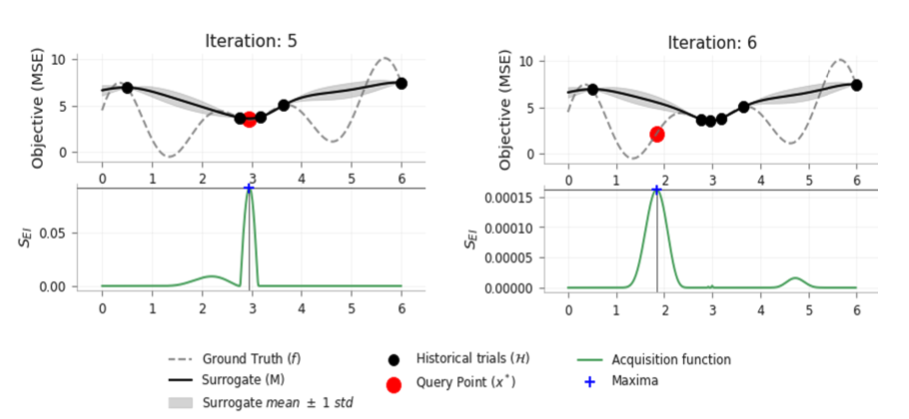
\includegraphics[scale=0.4]{figs/overview_bo.png}
	\refstepcounter{figure}
   	\addcontentsline{lof}{figure}{Figure~\thefigure: Illustration of Bayesian Optimization}
	\label{fig: bo}
	\parbox{\linewidth}{
	\vspace{0.5em}
 	{\small \textit{Figure \ref{fig: bo}:} Example of Bayesian optimization with Gaussian Process as the surrogate and \gls{ei} as the acquisition function to explore the minimum of the objective function \cite{agnihotri2020exploring}.
 	}
 	}
\end{figure}

Next, we return to the NAS framework "Bayesian optimization + neural predictor". Now it becomes obvious that this framework is essentially an optimization task that searches the maximum value. The objective function in this context maps each architecture in the search space to its corresponding validation accuracy. The surrogate model is a neural network and takes architectures or their encodings as the inputs. \cite{white2019bananas} identifies five critical components within the framework, listed as follows:

\begin{description}[leftmargin=0cm, listparindent=\parindent]
	\item [Architecture Encoding] This item refers to obtaining a vector representation of the architectures. Previous work often encode architectures using an adjacency matrix based approach, where nodes are assigned with an arbitrary ordering  and then binary features for all edges in the \gls{dag} are set to form the final representation.	Notably, the resulting representation of a specific architecture is not deterministic since the encoding  relies on an arbitrary indexing of the nodes. 
 
	In contrast, \cite{white2019bananas} proposes a novel path-based encoding mechanism with optional path truncation. This method simply checks if a path from the input node to the output node, expressed in terms of operations (e.g., input $\rightarrow$ 1$\times$1 conv $\rightarrow$ 3$\times$3 pool$\rightarrow$ output), is present in an architecture. The final encoding is a binary vector indicating which of the possible paths within a cell are present in the architecture. In this way, an architecture is always mapped to the same (though not necessarily unique) path encoding. Experiments show that the path-based encoding substantially increases the performance of neural predictors.
	
	\item [Neural Predictor] This item is about choosing an appropriate neural network for surrogate, which maps architecture encodings to the corresponding performances. To select the optimal neural predictor, several candidates are examined, include VAEs, GCNs, and FNNs with either adjacency matrix or path-based encoding. These predictors are first trained on a dataset, which is formed by randomly sampling a set of architectures and their corresponding validation accuracies from the search space, and then compared on holdout set. Among all tested neural predictors, FNNs with path encoding demonstrates the strongest performance.
	 
	\item [Uncertainty Estimation] Uncertainty estimates are required to form the probabilistic distribution. In particular, Bayesian neural networks (BNNs) and an ensemble of \gls{fnns} are investigated. For BNNs, the posterior distribution is inferred over the network weights. For \gls{fnns}, the predictive distribution is simply modeled as a Gaussian, parameterized by the mean and standard deviation of the ensemble base learners' predictions. The results show that an ensemble of even only 3 to 5 neural networks in general yields more reliable uncertainty estimates than BNNs.
	
	\item [Acquisition Function] In the experiments, five commonly used acquisition functions are examined: \gls{ts}, \gls{its}, \gls{ucb}, \gls{pi}, and \gls{ei}. Each function is adapted to the Gaussian assumption, thereby requiring only the mean and standard deviation estimates to compute the acquisition scores. The experiments show that overall \gls{its} yields the best performance among all the options, although the marginal outperformance is subtle. The results indicate that the acquisition function does not have as significant impact on the search performance as the other examined components in the framework.
		
	\item [Acquisition Optimization] In each iteration of the Bayesian optimization, the goal is to select a candidate from the search space that maximizes the acquisition score. Evaluating the acquisition function for every architecture available in the search space is computationally infeasible, therefore \cite{white2019bananas} proposes to create a set of 100 to 1000 candidates and then choose the architecture with the maximal acquisition score in this set. Specifically, \cite{white2019bananas} explores various approaches for creating this candidate set. The simplest and most natural way is to draw architectures at random. Consider that architectures close in edit distance to those used for training the surrogate model are likely to have more accurate estimates, an alternative is a mutation-based sampling approach, where the candidate set is created via local search by randomly modifying an operation or an edge of the best-performing architectures that have been evaluated so far. In additional, \cite{white2019bananas} also examines a hybrid approach that combines random search with mutation-based search. Their experiments show that the mutation-based approach outperforms its competitors and suggest it is better to search locally rather than globally.
\end{description}}

Finally, the best components found in the aforementioned analyses are transformed into the BANANAS algorithm. Considering its strength in both prediction and uncertainty quantification, an ensemble of \gls{fnns} using the path encoding is employed as the surrogate model and typically uncertainty is modeled as a Gaussian distribution. In addition, \gls{its} with a mutation strategy for acquisition (Figure \ref{fig: bananas}). 

\begin{figure}[t]
	\centering
	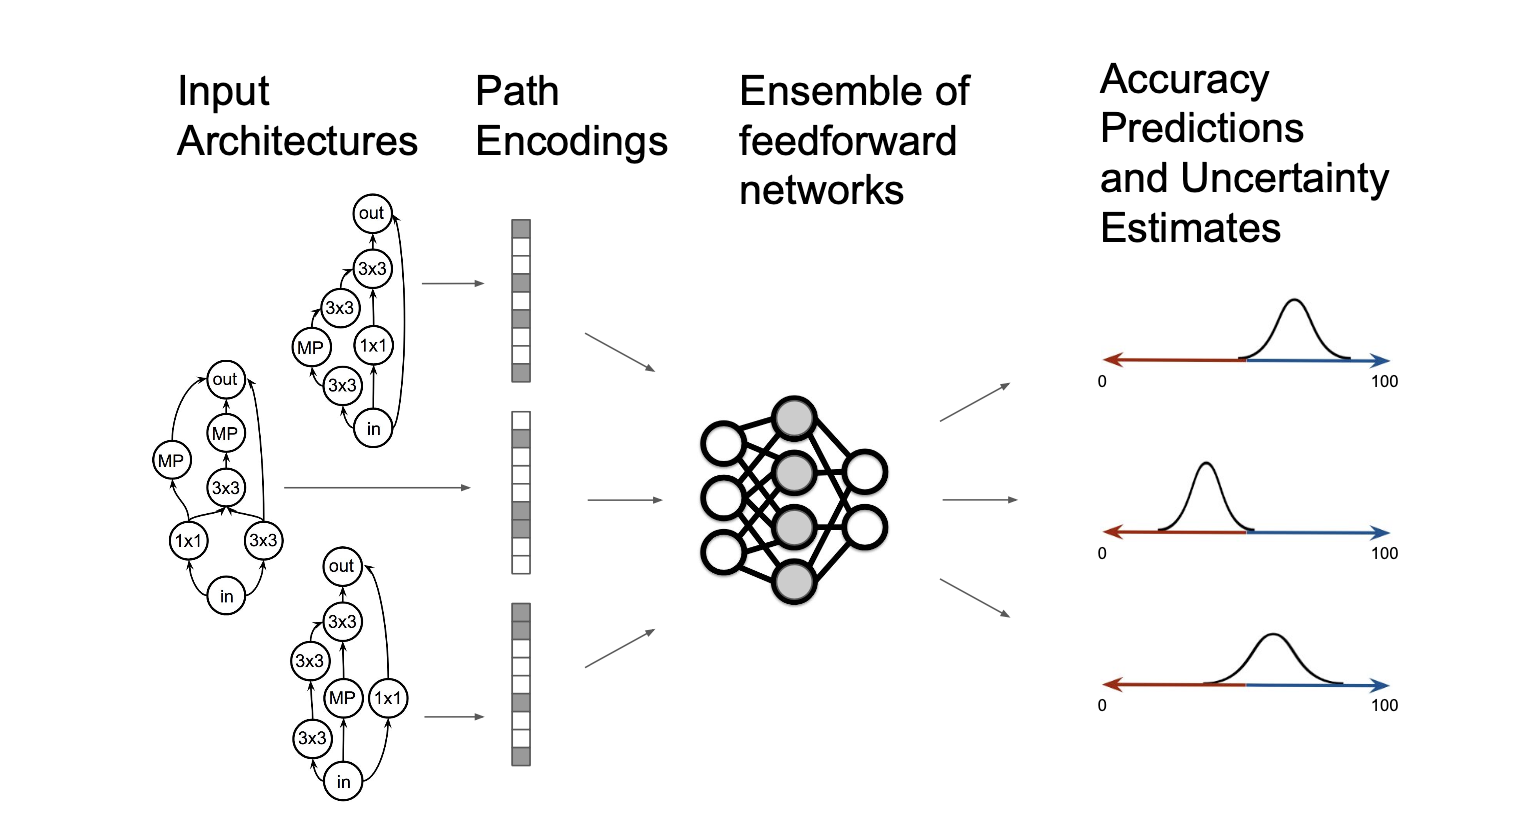
\includegraphics[scale=0.48]{figs/overview_bananas.png}
	\refstepcounter{figure}
   	\addcontentsline{lof}{figure}{Figure~\thefigure: Diagram of the BANANAS framework}
	\label{fig: bananas}
	\vspace{0.5em} 
	\\
 	{\small \textit{Figure \ref{fig: bananas}:} Diagram of the BANANAS framework \cite{white2019bananas}.}}
\end{figure}

\section{Uncertainty Quantification Methods}
While \gls{bananas} employs a relatively simple method for uncertainty estimation, there are many commonly used \gls{uq} techniques that are generally more theoretically grounded and sophisticated. In this section, we review some of these \gls{uq} methods and explain the rationale for choosing \gls{cp} for the development of our approach. Despite not directly tied to this work, this thesis aspires to offer a comprehensive overview of common \gls{uq} techniques applied in deep learning.

Formally, \gls{uq} is the science of quantitative characterization and estimation of uncertainties in both computational and real world applications. The source of uncertainty can be categorized into two types:

\begin{description}[leftmargin=0cm]
\item[Aleatory Uncertainty:] also known as data uncertainty, refers to uncertainty that arises due to inherent noices or randomness in a system and can not be reduced. \item[Epistemic Uncertainty:] also known as model uncertainty, refers to uncertainty that arises due to lack of knowledge, and can be reduced by better modeling or collecting more data.
\end{description}

A family of methods for quantifying uncertainty directly model the full predictive distribution of the output, i.e., $p(y \mid x)$. One example is the Gaussian Process, which is typically parameterized by a kernel function and the predictive inference can be obtained in an analytical manner based on the observations. Another important example is the Bayesian Neural Network \cite{kendall2017uncertainties, neal1996bayesian}, in which each weight in the network is seen as a random variable rather than a single number. In practice, however, the posterior distributions over weights are intractable due to the integral operation and the high dimensionality. Therefore, the posterior can only be approximated using e.g.,  variational inference or Monte-Carlo sampling methods \cite{neal1996bayesian, springenberg2016bayesian}, both requiring multiple forward passes through the network. 

Like the inference stage in BNNs, some methods also rely on aggregating statistics from sub-networks, such as Monte-Carlo Dropout \cite{gal2016dropout} and Deep Ensemble \cite{lakshminarayanan2017simple}. The idea of Monte-Carlo Dropout is to apply \textit{dropout}, a regularization technique often used for preventing overfitting during the training time by randomly deactivating neurons, also at the inference time. Specifically, the model run multiple times on the same input with stochastically deactivated neurons and thereby get  different predictions, which are seen as the approximation to the distribution of the output. Deep Ensemble involves using a network that outputs two values in the final layer, corresponding to the predicted mean $\mu(x)$ and the variance $\sigma^2(x)$, respectively. This neural network is typically trained by minimizing a custom loss function in which $\mu(x)$ and $\sigma^2(x)$ have opposing effects. To avoid overfitting and lower estimation variance, multiple instances of the neural network are initialized with different weights and trained independently. Then, the final estimates of $\mu(x)$ and $\sigma^2(x)$ are obtained by aggregating the predictions from all these sub-networks. 

Another popular approach is Quantile Regression (QR) \cite{koenker1978regression}. Instead of modeling the full distribution, QR only models a sequence of discrete quantiles of the output. We present QR with more details in Section \ref{sec:cp}. 

However, these \gls{uq} techniques face several challenges in practice. Some methods require multiple forward propagations either during the training or inference time, such as BNNs, Deep Ensemble. This is in general computationally intensive and may cause the models difficult to scale and consequently limit their applications for real-time prediction or in an online setting. In addition, the inference quality of BNNs depends on if the prior of weights is correctly specified, which demands expertise and can potentially introduce human bias. On the other hand, some models are pre-trained and are only accessible via API, making intervening the training process practically infeasible \cite{mossina2024CVPR}. Moreover, pre-trained models developed using certain datasets may struggle to generalize across different domains or contexts. 

\vspace{0.3cm}
Post-hoc uncertainty calibration techniques can serve as an effective approach in the restricted scenarios described above. Instead of assessing and measuring uncertainties on the model level, calibration targets on adjusting a model's predicted probabilities to make the reported uncertainties better aligned with the actual likelihoods.

Platt Scaling \cite{platt1999probabilistic} probably is the first calibration technique applied in modern machine learning. This method is introduced in the context of Support Vector Machines and is intended for classification problems. For regression problems, one widely used calibration technique is Isotonic Regression \cite{niculescumizil2005predicting}, a technique of fitting a step-wise line to a sequence of observations such that the fitted line is non-decreasing (or non-increasing) everywhere. The monotonicity of the resulting line allows to preserve the order of predicted quantiles, making this method appealing for uncertainty calibration. For example, \cite{pmlr-v80-kuleshov18a} show that accurate uncertainty estimates can be obtained by training a recalibrator on a holdout dataset using isotonic regression.

Recently, Conformal Prediction (CP) \cite{shafer2008tutorial, vovk2005algorithmic} is emerged as a new, distribution-free framework for uncertainty quantification. This technique has been widely adopted for both classification and regression problems despite of its relatively short history. Fundamentally, CP serves as a model-agnostic wrapper and can be applied with any arbitrary prediction algorithms. It works by constructing a prediction interval (for regression) or a set of possible values (for classification) that will cover the true value with a predefined probability. The fact that \gls{cp} is applied in a post-hoc fashion with minimal assumptions enables it to capture both aleatoric and epistemic uncertainties \cite{mossina2024CVPR}. Moreover, like most other post-hoc calibration methods, \gls{cp} offers the advantage of being light-weighted with little overhead to implement. We present a thorough introduction into the \gls{cp} framework in the following section.

\section{Conformal Prediction}
\label{sec: reviewCP}
\subsection{Theoretical Background}
We start by introducing the concept of \textit{exchangeable data}, which is an key prerequisite for understanding \gls{cp}.
\newline

\noindent
\textbf{Definition (Exchangeability):}  
A sequence of random variables \( (Z_1, Z_2, \dots, Z_n) \) is said to be \textit{exchangeable} if its joint probability distribution is invariant under any permutation of the indices. That is, for every permutation \( \pi \) of the set \( \{1, 2, \dots, n\} \),
\[
P(Z_1, \dots, Z_n) = P(Z_{\pi(1)}, \dots, Z_{\pi(n)})
\]

\noindent Note that exchangeability allows for dependencies among data points, as long as the joint distribution is invariant under any permutation. Accordingly, it is weaker than the i.i.d. assumption. Then, the goal of \gls{cp} can be formally defined as: 
\newline

\noindent
\textbf{Definition (Conformal Prediction):}  Let \(B = \{(x_1, y_1), \dots, (x_n, y_n)\}\) be a bag of observed examples from an exchangeable joint distribution $\mathbb{P}_{X,Y}$, with $X \subset R^d$ representing some features and  $Y$ the target variable. Given a new unseen input \(x_{n+1}\), conformal prediction constructs a prediction region \( \mathcal{C}_n^\tau(x_{n+1}) \) using a \textit{conformity score function} such that
\vspace{0.7em}

\begin{equation}
\mathbb{P}\left( y_{n+1} \in \mathcal{C}_n^\tau(x_{n+1}) \right) \geq 1 - \tau
\vspace{1em}
\label{eq: finitecp}
\end{equation}

\noindent
where \( \tau \in (0, 1) \) is the predefined nominal mis-coverage rate. This probability is also known as the \textbf{finite-sample validity} property of \gls{cp} and is taken over the joint distribution of all \(n + 1\) samples. Moreover, the prediction regions for different $\tau$ should be nested. That means, if  $\tau_1 \ge \tau_2$, then $1 - \tau_1$ is a lower confidence level than $1 - \tau_2$ and we have $ \; \mathcal{C}_n^{\tau_1}(x_{n+1}) \subseteq \mathcal{C}_n^{\tau_2}(x_{n+1})$ \cite{shafer2008tutorial}.  

\vspace{0.7em}
\textbf{Conformity score function} is a real-valued function  measures how dissimilar the unseen example $x_{n+1}$ is compared to the existing examples in the bag $B$. Now generalizing this setting to a supervised learning framework, a predictive algorithm $f$ that maps features to the target variable naturally induces a conformity measure. Specifically, we denote $\hat{f}_n$ the predictor trained on the $n$ existing observations in the bag and $d(z_{n+1}, B), \; z_{n+1} = (x_{n+1}, y_{n+1})$ the conformity function, such that a higher value indicates a greater deviation of the new sample from the existing ones. When using $\hat{f}_n$ to generate a point prediction for $x_{n+1}$, since the prediction rule is learnt from examples in the bag, intuitively, the distance between the predicted value $\hat{f}_n(x_{n+1})$ and the true value $y_{n+1}$ informs how different $z_{n+1}$ is compared to the rest examples in the bag. With a conformity score function of this kind, the prediction set is constructed by collecting all values that lie within a certain distance from the true value, i.e., all values such that $d(\cdot, B)$ smaller than a threshold.

\begin{figure}[H]
	\centering
	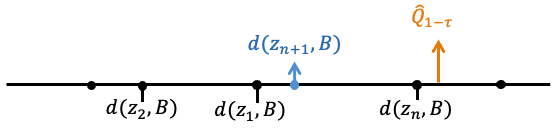
\includegraphics[scale=0.35]{figs/cp_symmetry.png}
	\refstepcounter{figure}
   	\addcontentsline{lof}{figure}{Figure~\thefigure: Illustration of Symmetrical Data}
	\label{fig: cpsymmetry}
	\vspace{0.5em} 
	\\
 	{\small \textit{Figure \ref{fig: cpsymmetry}:} Illustration of Symmetrical Data in Conformal Prediction}}
\end{figure}

\vspace{0.5em} 
An important intuition behind selecting the threshold that eventually defines the prediction region is \textit{symmetry}, that is, all data points are treated symmetrically within the \gls{cp} framework \cite{angelopoulos2021gentle}. Suppose $d(z_1, B), \, d(z_2, B), \; ... \; ,d(z_n, B)$ is a sequence of observations in the form of conformity scores, the exchangeability assumption implies that the rank of a new data point $d(z_{n+1}, B)$ is uniformly distributed over the observed values. Figure \ref{fig: cpsymmetry} illustrates the concept of symmetry, in which the new data point is equally likely to take any value on the number line. As a result, the $(1 - \tau)$-th quantile of all the conformity scores is a natural answer to achieve the coverage probability stated in Formula \ref{eq: finitecp}. Recall that the coverage probability is achieved on the $n+1$ samples, the quantile value should be adjusted with a finite-sample correction, resulting in a threshold that is exactly equal to 

\begin{equation}
\vspace{0.7em}
\frac{\lceil(1 - \tau)(n + 1)\rceil}{n}\text{-th quantile of conformity scores}
\label{eq:cpquantile}
\vspace{0.7em}
\end{equation}

\noindent
\textbf{Finite-sample Validity} Note that the coverage guarantee provided by the \gls{cp} framework is marginal, meaning it holds on average over all data points. This is a significantly weaker requirement than the conditional coverage, which requires the guarantee to hold for each individual input (Figure \ref{fig: coverage}). Nevertheless, \gls{cp} remains a powerful tool for uncertainty quantification, because the finite-sample coverage is valid regardless of the size of the observations bag or the choice made for the underlying prediction algorithm or the conformity score function. Under the distance interpretation presented earlier, a smaller score indicates that the new sample conforms more closely with the existing observations. In such case, the function is also referred as a negatively-oriented score and, to be precise, it is actually a non-conformity measure. A positively-oriented one also works in practice, provided with correct modifications. 

\begin{figure}[htbp]
	\centering
	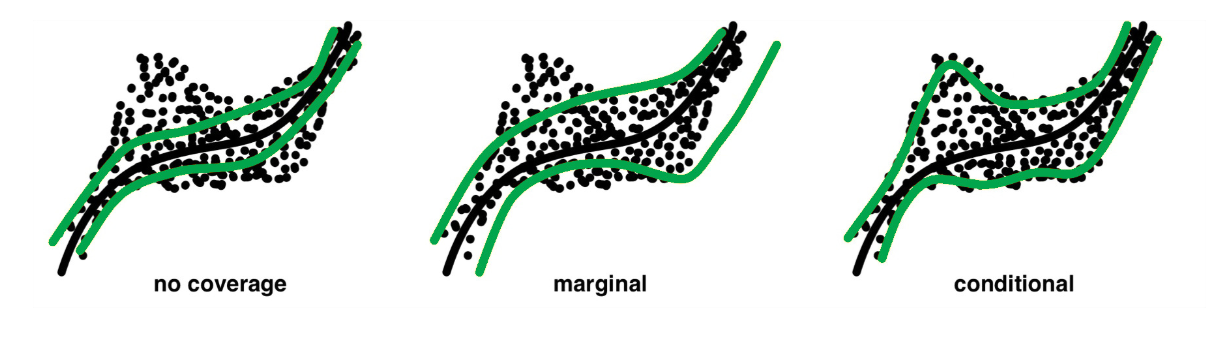
\includegraphics[scale=0.28]{figs/overview_coverage.png}
	\refstepcounter{figure}
   	\addcontentsline{lof}{figure}{Figure~\thefigure: Example of Different Coverage Types}
	\label{fig: coverage}
	\vspace{0.5em} 
	\\
 	{\small \textit{Figure \ref{fig: coverage}:} Example of Different Coverage Types}}
\end{figure}

Although coverage is guaranteed for any conformity scoring function, this scoring method is actually an important engineering decision and has significant impact on the effectiveness of the constructed prediction set. Imagine a classification problem, if we produce a set that contains all possible classes, then surely the true label is covered by the set. However, such prediction set is neither informational nor actionable, offering little value in application. This concern naturally introduces a second evaluation criterion for \gls{cp}: while ensuring coverage guarantees, ideally the yielded prediction set should be as compact as possible.

\vspace{1.5em}
\noindent \textbf{A Link to Hypothesis Testing} It is noticeable that \gls{cp} exhibits a couple of structural similarities to hypothesis testing, which is a fundamental tool in statistical inference and perhaps sounds more familiar to most ears. For example, both methods involves producing an interval and relying on a certain threshold to make decisions. In fact, these terms are often used interchangeably in many research work. This motivates us to seek an interpretation of the \gls{cp} framework through the hypothesis testing perspective, such that we gain a deeper and clearer understanding of \gls{cp}.

\begin{table}[t]
    \centering
    \refstepcounter{table}
   	\addcontentsline{lot}{table}{Table~\thetable: Comparison between Conformal Prediction and Hypothesis Testing}
   	
 	{\small \textit{Table \ref{tab:cpht_comparison}:} Comparisons between conformal prediction and hypothesis testing}
	\vspace{0.7em}

    \renewcommand{\arraystretch}{1.2}
   	\begin{tabular}{| m{1.5cm} | m{6cm} | m{5.8cm} |}
    \hline
    &\textbf{Conformal Prediction} & \textbf{Hypothesis Testing} \\
    \hline
    \textbf{Input} & nominal mis-coverage level $\tau$ & significance level $\alpha$ \\
    \hline
    \textbf{Decision rule} & compare the conformity score of a data point against the quantile value & compare $p$-value, which is an empirical measure, to the significance level \\ 
    \hline
	\textbf{Output} & prediction interval offering marginal coverage with probability $1 - \tau$ & confidence interval that contains the true parameter value with probability $1 - \alpha$  \\
	\hline        		
    \end{tabular}
    \label{tab:cpht_comparison}
\end{table}
	  	
Both methods take a predefined value ranging from 0 to 1 as input. In the context of \gls{cp}, this value is often interpreted as mis-coverage rate or error rate, referring to the probability that the prediction region fails to cover the true value. The corresponding concept in hypothesis testing is the significance level, referring to the probability of rejecting the null hypothesis when it is actually true. Table \ref{tab:cpht_comparison} offers a summary of the terms used in \gls{cp} alongside with their parallel in hypothesis testing.

Intuitively, we can think \gls{cp} as running a sequence of hypothesis tests for a given new point $x_{n+1}$, with each testing a candidate value for $y_{n+1}$, denoted as $\tilde{y}$. Hypotheses are defined as: \\

\vspace{-0.3em}
\indent $H_0$: The new example $(x_{n+1}, \; \tilde{y})$ conforms to the existing observations. \\
\indent	$H_1$: The new example $(x_{n+1}, \; \tilde{y})$ does not conform to the existing observations. \\
\vspace{-0.3em}

\noindent After obtaining conformity scores for all $n+1$ data points, in this context, the fraction of conformity scores that is larger than that for $(x_{n+1}, \tilde{y})$, or equivalently, the complement of the quantile of the conformity score for $(x_{n+1}, \tilde{y})$, can be seen as a $p$-value. If the $p$-value exceeds the predefined significance level, we fail to reject the null hypothesis, and consequently, this candidate $\tilde{y}$ is included in the prediction set. In fact, this interpretation from the hypothesis testing perspective reflects the core idea of the approach known as full conformal prediction, which we formally introduce in the following section.

\subsection{Full Conformal Prediction}
In fact, conformal prediction is originally designed for a transductive setting, in which the prediction for a test point is generated using the full dataset available at the inference time \cite{gammerman1998learning}. Hence, this transductive \gls{cp} framework is also known as \gls{fcp}. Typically, new observations are revealed sequentially, which means, after the prediction is generated for a test point, its true value is observed before the next prediction is made. 

The core idea for constructing a prediction set for a given test point $x_{n+1}$ is to iterate over all possible values in the target variable space. As performed in hypothesis testing, for each candidate $\tilde{y}$, a conformity score and its corresponding $p$-value will be calculated. Specifically, the conformity score for candidate $\tilde{y}$ is computed in a way where a prediction rule $\hat{f}_{\tilde{y}}$ is learnt using all pairs in the bag \(B = \{(x_1, y_1), \dots, (x_n, y_n), (x_{n+1}, \tilde{y})\}\), then the conformity score is computed as a distance measure between $\hat{f}_{\tilde{y}}(x_{n+1})$ and $\tilde{y}$. This process is repeated for all available candidates and the prediction set is constructed by collecting every $\tilde{y}$ with which the null hypothesis in the previous sub-section can not be rejected. Typically, if the target variable space is continuous, the space is first discretized to form a finite grid, then each element in the set can be checked, e.g., using grid search \cite{angelopoulos2021gentle}.

Moreover, after the true value $y_{n+1}$ is revealed, the underlying bag of observations gets updated by including this data point, and the above procedure needs to start from scratch when generating prediction for each new test point. Suppose the target variable space has a size of $K$, to generate prediction regions for $m$ instances, the underlying prediction algorithm should fit for $K \cdot m$ times. Clearly, \gls{fcp} in general is extremely computationally expensive, which renders the application of \gls{fcp} highly unsuitable for training-intensive works, such as with neural networks.

\subsection{Extensions of Conformal Prediction}
Since the transductive version of \gls{cp} that was first proposed in \cite{gammerman1998learning}, several variants of \gls{cp} have been developed with different computational complexities, formal guarantees, and practical applications.

To address the aforementioned inefficient computation problem of \gls{fcp}, Split Conformal Prediction (\gls{scp}), also known as Inductive Conformal Prediction (ICP), was first introduced in \cite{papadopoulos2002inductive} by replacing the transductive inference with inductive inference, aiming to learn a general prediction rule about the data using the observed records. Then, this rule can be applied directly to obtain predictions when new data arrives in sequence, without re-using the training data and retraining the model repeatedly. The main concept involves splitting the data into two non-overlapping subsets, designated for training and calibration, respectively. A predictive model is fit exclusively on the training set, then (non-)conformity scores are computed using the calibration set to obtain the quantile value that determines the width of the prediction interval. Due to its simplicity and computational efficiency, \gls{scp} is one of the most commonly used techniques in the \gls{cp} family. We introduce the methodological steps of \gls{scp} in details with pseudo-code in Section \ref{sec:scp}.

\vspace{0.5em} 	
Apart from hight computational cost, \gls{cp} still faces several challenges in practice: 
\vspace{0.2em} 

\noindent \textbf{Distribution/Covariate Shift:} The finite-sample validity offered by \gls{cp} depends on exchangeable data. However, the key assumption of exchangeability is often violated in real-world applications, in which the underlying data generation process might vary over time. For example, in finance market behavior can shift drastically in response to major world events. \\
 \noindent \textbf{Adaptivity:} The conformity score adopted in the original \gls{scp} work is based on the  absolute residual $|y - \hat{y}|$, which leads to a prediction interval with fixed width and does not adapt to the intrinsic complexity of the specific test example.
\vspace{0.5em} 

Various \gls{cp} algorithms have been developed to address limitations and broaden application domains. These extended algorithms can be mainly categorized into three types in accordance with the structural components in a \gls{cp} framework. 
\vspace{0.5em} 

One line of work focus on the coverage rate. Instead of using a static predefined mis-coverage rate $\tau$ for computing the quantile of conformity scores, \cite{gibbs2021adaptive} develops a method called \textit{ACI} where the applied coverage level is dynamically adapted based on empirical mis-coverage frequency of previous prediction sets. This approach is applied in an online setting. At each time $t$, the applied coverage rate $\tau_t$ is derived by decreasing (resp. increasing) the current value if the prediction sets were historically under-covering (resp. over-covering). The amplitude of rate adjustment is jointly controlled by the pre-specified learning rate and the empirical mis-coverage level. As an example, if the preset target coverage rate is 90\%, historical coverage rate suggests the applied coverage should set to 93\%, then this adjusted value is used for computing quantile. In this setting, the empirical mis-coverage frequency of previous examples serves as a signal of distribution shift or violation of exchangeability. \cite{gibbs2021adaptive} show that \textit{ACI} is capable of forming prediction sets that are robust to changes in the underlying data distribution. \cite{zaffran2022adaptive} extends \textit{ACI} to time-series data and introduce \textit{AgACI}, which is a parameter-free variant of \textit{ACI} that uses online expert aggregation to adaptively combine multiple ACI experts. In contrast to \textit{ACI}, where the learning rate should be carefully chosen in advance, \textit{AgACI} leverages a number of $k$ experts working with different learning rates, and automatically learns the optimal learning rate by aggregating across experts such that each expert's contribution is proportional to their corresponding performances over previous iterations. \cite{zaffran2022adaptive} show \textit{AgACI} demonstrates strong performance and produces tighter, well-calibrated prediction intervals consistently.  
\vspace{0.5em} 

Another line of work strives to find suitable and efficient conformity score functions tailored for specific tasks. For example, \cite{lei2018distribution} introduces a simple score for regression that accounts for heteroskedasticity, thus offering local adaptivity. \cite{romano2020classification} proposes a novel conformity score crafted for multi-label classification tasks. While providing marginal coverage, this score also demonstrates full adaptiveness to data complexities and enhances the approximated conditional coverage. In parallel, \cite{romano2019conformalized} develops a conformity score that involves both upper and lower bounds corresponding to a given coverage rate, enabling to combine the strengths of quantile regression and conformal prediction. Furthermore, \cite{xie2024boosted incorporates a boosting procedure between the training and calibration steps in order to enhance an arbitrary score function.

\vspace{0.5em} 
The underlying prediction algorithm also plays an important role in \gls{cp}, since the trained predictor serves as an approximation of the real data generation process and determines the base from which intervals are constructed. \gls{scp} fits the predictor only once, however potentially at a cost of training accuracy and  but statistical efficiency, since both training set and calibration set only see a subset of samples. One way to address this challenge is combining conformal prediction with techniques like cross-validation\cite{vovk2015cross}, Jackknife+ \cite{barber2020jackknife} and bootstrapping \cite{kim2020predictive}, such that all data points are used for both training and calibration, with only a limited number of model fits. 

\vspace{0.5em} 
In addition, there are works beyond the above three categories. Some works boost prediction reliability through enhancing the datasets. \cite{StutzTMLR2023} proposes a CP algorithm targeted on a special classification case where the ground-truth is ambiguous and consequently cause a biased distribution in manually-annotated labels. This method approximates the true distribution of labels by resampling data points using Monte-Carlo sampling. \cite{Shanmugam2025TTA} proposes to integrate a test-time data augmentation into \gls{cp} to reduce prediction set size and improve stability. Moreover, Conformal Risk Control \cite{angelopoulos2022conformal} also emerges as an important extension of \gls{cp} that not only provides distribution-free coverage guarantees but also explicitly controls risk. It is achieved by replacing the mis-coverage probability in normal \gls{cp} with the expected value of a custom loss function. The prediction set is then bounding to the predefined loss tolerance instead of the mis-coverage rate. Several works have adopted this risk-control approach such as \cite{mossina2024CVPR}.
